\documentclass[12pt]{scrartcl}
\input{NiaLatexHelpers/nia_defs.tex}

\title{\vspace{-2em} Logic with Numbers and Strings}
\author{}
\date{}

\newcommand{\pyTrue}{\pythonl{True}\xspace}
\newcommand{\pyFalse}{\pythonl{False}\xspace}


\begin{document}
\maketitle
\vspace{-6em}
\section{Breaking Problems Into Cases}
We've been working on functions that take in \pyTrue{}s and \pyFalse{}s and spit out \pyTrue or \pyFalse.
\begin{figure}[H]
    \centering
    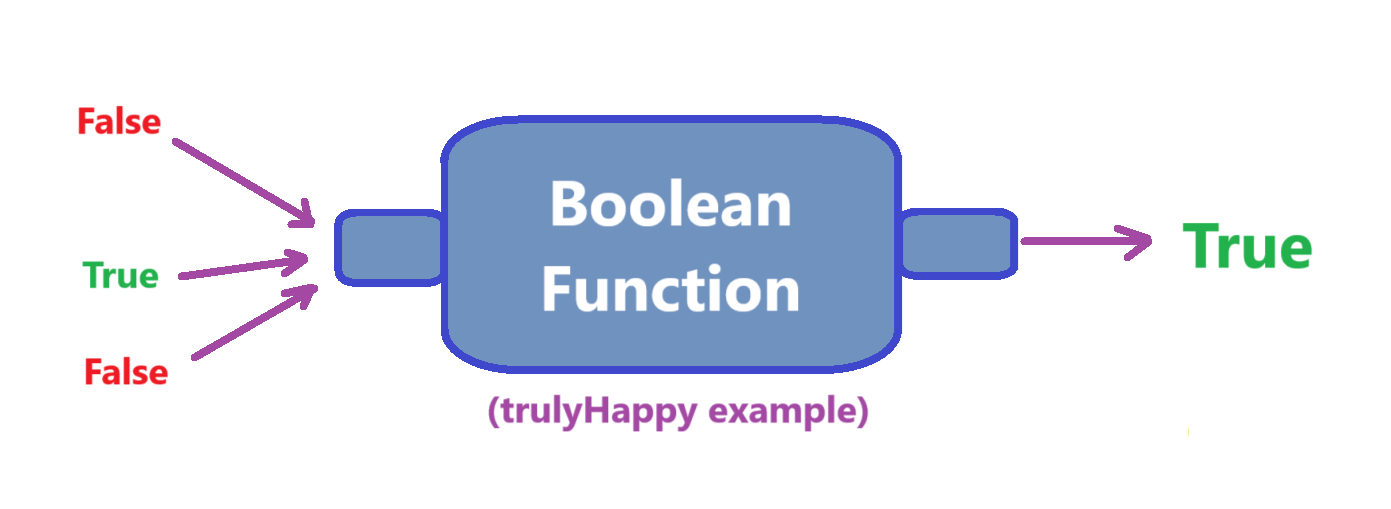
\includegraphics[scale=0.3]{Boolean Functinos.png}
    \caption*{\pythonl{trulyHappy} was a problem from the previous homework.}
\end{figure}
In these problems, because we only had \pyTrue and \pyFalse as inputs, the amount of possibilities we had to handle was small. But what if we took in numbers as inputs? Then there would be infinite cases to handle for every possibility! 
\begin{python}
def function(num):
    if num == 0:
        (Code)
    if num == 1:
        (Code)
    if num == 2:
        (Code)

    |...And so on!!|
\end{python}
For example, what if we wanted to write a function where if the input number was even, we return twice the number, and if the number is odd, we return thrice the number. It might be tempting to write:
\begin{python}
    def coolFunction(num):
        if num == 0:
            return 0  |\qquad $(2\cdot 0)$|
        if num == 1: 
            return 3  |\qquad $(3 \cdot 1)$|
        if num == 2:
            return 4  |\qquad $(2 \cdot 2)$|
        if num == 3
            return 9  |\qquad $(3 \cdot 3)$|
        if num == 4
            return 8  |\qquad $(2 \cdot 4)$|
        if num == 5
            return 15 |\qquad $(3 \cdot 5)$|
        

        |... And so on!|
\end{python}
But this would be infinite code to have to write. Instead, what if we just wrote code to handle if the number is odd and code to handle if the number is even? Reminder that the \% operator in Python gets the remainder. We can think of what we have to do in the following chart:
\begin{center}
\begin{tabular}{c|c|c}
    Input & If Statement & Output \\
    \hline
    \pythonl{num} is even & \pythonl{if num |\%| 2 == 0} & \pythonl{2 * num} \\
    \pythonl{num} is odd & \pythonl{if num |\%| 2 == 1} & \pythonl{3 * num}
\end{tabular}
\end{center}
Therefore, our code would be:
\begin{python}
    def coolFunction(num):
        if num % 2 == 0:
            return 2 * num
        elif num % 2 == 1:
            return 3 * num
\end{python}
That's a lot better than infinite code to write! You can see the power of cases here. Via cases, we could handle every number possible, just like how we could handle every possible input of \pyTrue and \pyFalse in boolean problems.

\section{Practice with a CodingBat Problem}
Let's look at \codel{Warmup-1 |$\to$| sum_double}:

\begin{callout}
    Given two int values, return their sum. Unless the two values are the same, then return double their sum.

    Example:
    \begin{purecode}
    sum_double(1, 2) |$\to$| 3
    sum_double(3, 2) |$\to$| 5
    sum_double(2, 2) |$\to$| 8
    \end{purecode}
\end{callout}

If we handled every possible input, we would have $\infty$ numbers times $\infty$ numbers equals $\infty$ possibilities. But once again, we can divide into cases:
\begin{center}
    \begin{tabular}{c|c|c}
        Input & If Statement & Output \\
        \hline
        \pythonl{a} and \pythonl{b} are different & \pythonl{if a != b} & \pythonl{a + b} \\
        \pythonl{a} and \pythonl{b} are the same & \pythonl{if a == b} & \pythonl{2 * (a + b)}
    \end{tabular}
\end{center}
In programming, to say $a \neq b$, we say \pythonl{a != b}, which is what we have above. We can use this chart to write our solution:
\begin{python}
    def sum_double(a,b):
        if a == b:
            return 2 * (a + b)
        elif a != b:
            return a + b
\end{python}
Notice that we can simplify this code into:
\newpage
\begin{python}
    def sum_double(a,b):
        if a == b:
            return 2 * (a + b)
        else:
            return a + b
\end{python}
Because \pythonl{return} immeadetly ends a function, we don't really need the \pythonl{else} here first, meaning the code can be further simplified into:
\begin{python}
    def sum_double(a,b):
        if a == b:
            return 2 * (a + b)
        return a + b
\end{python}
Here, we handle the exception first (the numbers are exactly the same), and then we handle the main case (where the numbers are different, which is the majority of the time) afterwards.

\section{Sometimes We Don't Need Cases}
Consider this problem:
\begin{callout}
    Write a function \pythonl{explode} that takes in two numbers $a$ and $b$ and returns the sum of $a^b$ and $b^a$.
\end{callout}
There's only one scenario here: no matter what the inputs are, we always return $a^b + b^a$. So our code isn't:
\begin{python}
    def explode(a,b):
        if (a == 0 and b == 0):
            return 0**0 + 0**0
        if (a == 0 and b == 1):
            return 0**1 + 1**0
        if (a == 1 and b == 0):
            return 1**0 + 0**1
        
        |...and so on.|
\end{python}
Instead, our code is:
\begin{python}
    def explode(a,b):
        return a**b + b**a |\qquad (This handles every scenario!!)|
\end{python}

Try to break a problem down into the main scenarios. Is there an equation that relates the input to the answer? Or do you need multiple equations depending on the input, requiring cases?

\section{Logic with Strings}
Just like how we could handle problems with numbers as inputs, we can also handle problems with strings (English words) as inputs. Despite how there's infinite possibilities of input---as there's infinite English sentences you could give as input---we can still break a problem into cases (or potentially solve it without cases). Consider CodingBat problem \codel{String-1 |$\to$| make_abba}:

\begin{callout}
    Given two strings, a and b, return the result of putting them together in the order abba, e.g. \codel{"Hi" |and| "Bye"} returns \codel{"HiByeByeHi"}.

    \begin{purecode}
        make_abba('Hi', 'Bye')   |$\to$| 'HiByeByeHi'
        make_abba('Yo', 'Alice') |$\to$| 'YoAliceAliceYo'
        make_abba('What', 'Up')  |$\to$| 'WhatUpUpWhat'
    \end{purecode}
\end{callout}

First, notice that in Python, we can use \pythonl{'} and \pythonl{"} interchangably. This isn't the case in other langauages, but for Python, it's totally okay to say \pythonl{"cat"} or \pythonl{'cat'}: both are strings and are the same thing to the computer.

Let $a$ and $b$ represent the input strings. No matter what $a$ and $b$ are, we always return $a + b + b + a$. So our code shouldn't be:
\begin{python}
    def make_abba(a,b):
        if a == "Hi" and b == "Bye":
            return "HiByeByeHi"
        if a == "Yo" and b == "Alice":
            return "YoAliceAliceYo"
        if a == "What" and b == "Up:
            return "WhatUpUpWhat"
        
        |...and so on forever.|
\end{python}
Instead, our code is:
\begin{python}
    def make_abba(a,b):
        return a + b + b + a
\end{python}
and this code will handle every scenario! Trust that the algebra will work for any input. Your computer is smart. It can do it even if it looks like variables to you.

\section{Tools to Help Us with Numbers}
For comparing numbers and writing if-statements, there's a lot of useful operators:
\begin{center}
    \begin{tabular}{c|c}
        Operator & Math Meaning \\
        \hline
        \pythonl{a == b} & $a = b$ \\
        \pythonl{a != b} & $a \neq b$ \\
        \pythonl{a < b} & $a < b$ \\
        \pythonl{a <= b} & $a \leq b$ \\
        \pythonl{a > b} & $a > b$ \\
        \pythonl{a >= b} & $a \geq b$
    \end{tabular}
\end{center}
These operators all give an output of \pyTrue whenever the math equation is correct. So \pythonl{4 < 5} would be \pyTrue, so the following if-statement
\begin{python}
    a = 4
    b = 5
    if a < b:
        (Code)
\end{python}
The code inside the \pythonl{if} would indeed happen. Similarly, \pythonl{3 >= 3} as $3 = 3$, so the code
\begin{python}
    c = 3
    d = 3
    if c >= d:
        (Code)
\end{python}
would also have its code run.

\section{Tools to Helps Us with Strings}
Just like with numbers, we can use \pythonl{== |and| !=} to compare strings. But there's other operations as well. Consider the following string:
\begin{center}
    \pythonl{s = "a racecar"}
\end{center}
Including the spaces, there are 9 characters (called \pythonl{char}s in programing) in this string:
\begin{figure}[H]
    \centering 
    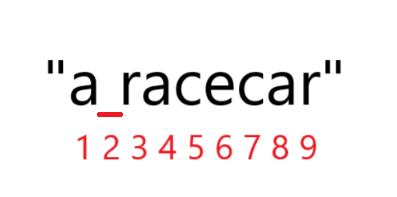
\includegraphics[scale=0.5]{A racecar Counted.png}
    \caption*{A line is put under the space in this diagram for counting purposes.}
\end{figure}
To get a letter from a string \pythonl{s}, you write \pythonl{s[i]}, replacing $i$ with the number of the letter you want. However, if you actually tried \pythonl{s[3]}, you would get \pythonl{'a'} and not \pythonl{'r'} as expected. This is because in programming, we count strings starting with the first letter as index 0. We start at 0 because it was easier to build early computers this way. So here is a diagram of the letters correctly numbered:
\begin{figure}[H]
    \centering 
    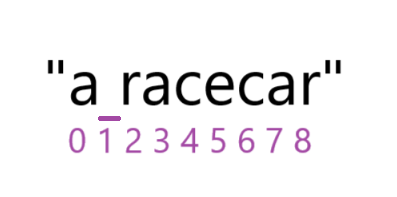
\includegraphics[scale=0.5]{A racecar Indexed.png}
    \caption*{Notice that \pythonl{s[2]} is \pythonl{'r'}, not \pythonl{s[3]}.}
\end{figure}
To get a section from a larger string, we do \pythonl{s[i:j]}. So for example, \pythonl{s[2:2+4]} would be the string \pythonl{"race"}. This is called a \textit{substring}.

I wrote $2 + 4$ because there's four letters in race. Since $2+4 = 6$, we could have also written \pythonl{s[2:6]}. But notice that \pythonl{s[6] == 'c'}, not \pythonl{'e'}! So when we find substrings, we give the index of the first letter and then the index of the letter\\ \textit{one after} we want to stop at. So as another example:

\begin{center}
    \pythonl{s[6:9] == "car"}
\end{center}

To get the length of a string, we use \pythonl{len()}. So here, \pythonl{len(s) == 9}. This means we could also have written:

\begin{center}
    \pythonl{s[6:len(s)] == "car"}
\end{center}

To summarize,

\begin{center}
    \begin{tabular}{c|p{7cm}}
        Code & Meaning \\
        \hline
        \pythonl{a == b} & Are \pythonl{a} and \pythonl{b} the same words. \\
        \pythonl{a != b} & Are \pythonl{a} and \pythonl{b} different words. \\
        \pythonl{s[i]} & The $i$th $+\:1$ letter. \\
        \pythonl{s[i:j]} & The substring starting at index $i$ and ending one before index $j$. \\
        \pythonl{len(s)} & The length of the string \pythonl{s}.
    \end{tabular}
\end{center}

There's a lot more we can do with strings, but we'll learn about them in a future lesson.

Let's use what we learned to solve a problem. Consider the following CodingBat problem, which is \codel{String-1 |$\to$| without_end}
\begin{callout}
    Given a string, return a version without the first and last char, so \pythonl{"Hello"} yields \pythonl{"ell"}. The string length will be at least 2.
    
    \begin{purecode}
        without_end('Hello') |$\to$| 'ell'
        without_end('java') |$\to$| 'av'
        without_end('coding') |$\to$| 'odin'
    \end{purecode}
\end{callout}
You might be tempted to handle every possibility:
\begin{python}
    def without_end(s):
        if s == "Hello":
            return "ell
        if s == "python":
            return "ytho"
        if s == "cute cat":
            return "ute ca"
        
        ...And so on forever.
\end{python}
But that would be infinite code to write to handle every possible English string of words! Instead, we can recognize there's only \textbf{one case}: remove the first and last letters, which we can do with substrings.

We want to skip the first letter, which is letter 0, meaning we should start at 1. And we want to skip the last letter. The last letter of any string is \pythonl{len(s) - 1}: For example, 
\begin{python}
    def without_end(s):
        return s[1:len(s)-1]
\end{python}

\section{Homework}
It's time for CodingBat! Here's what I would like you to do:

\textbf{Numbers:}
\begin{enumerate}
    \item \codel{Warmup-1 |$\to$| parrot_trouble}
    \item \codel{Warmup-1 |$\to$| diff21}
    \item (A step up) \codel{Warmup-1 |$\to$| makes10}
    \item (Challenging) \codel{Warmup-1 |$\to$| near_hundred}
\end{enumerate}

\medskip

\textbf{Strings:}
\begin{enumerate}
    \item \codel{String-1 |$\to$| hello_name} 
    \item \codel{String-1 |$\to$| extra_end}
    \item \codel{String-1 |$\to$| first_two}
    \item \codel{String-1 |$\to$| first_half}
    \item (A step up) \codel{String-1 |$\to$| make_out_word}
    \item (Similar difficulty) \codel{String-1 |$\to$| make_tags} 
\end{enumerate}

\end{document}